\section{PROCEDIMIENTO} 


\begin{enumerate}[1.]
	\item Escribiendo consultas con el operador PIVOT
	\begin{enumerate}[a)]
	\item Paso 1: Escribir una sentencia SELECT para recuperar el numero de clientes para un grupo especifico de clientes.\\
		-  Abrir el SQL Server Management Studio y conectar a la basa de datos (local) usando Windows.\\
		-  Usar la base de datos TSQL\\
		-  Ejecutar el siguiente codigo para crear una vista\\
		\begin{figure}[H]
		\begin{center}
		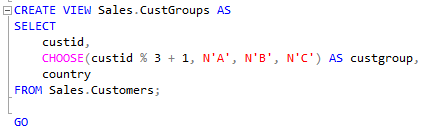
\includegraphics[width=8cm]{./Imagenes/1-1}
		\end{center}
		\end{figure}
		-  En el panel de consulta, escribir la siguiente consulta.
		\begin{figure}[H]
		\begin{center}
		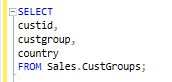
\includegraphics[width=6cm]{./Imagenes/c1}
		\end{center}
		\end{figure}
		-  Luego modificamos el codigo, aplicando el operador PIVOT.
		\begin{figure}[H]
		\begin{center}
		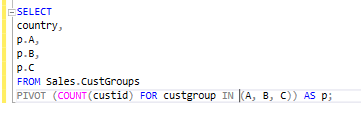
\includegraphics[width=6cm]{./Imagenes/c2}
		\end{center}
		\end{figure}
	\item Paso 2: Especifique el elemento de agrupacion para el operador PIVOT. \\
		-  Escribir la siguiente consulta para poder modificar la vista creada anteriormente, añadiendo 2 columnas adicionales. 
		\begin{figure}[H]
		\begin{center}
		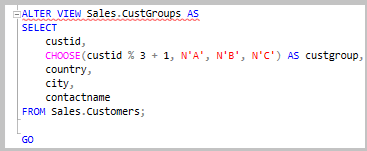
\includegraphics[width=7cm]{./Imagenes/e1-2}
		\end{center}
		\end{figure}
		-  Escribir la siguiente consulta. 
		\begin{figure}[H]
		\begin{center}
		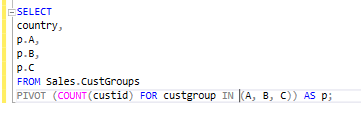
\includegraphics[width=6cm]{./Imagenes/c2}
		\end{center}
		\end{figure}
		-  Modificar la consulta para incluir columnas adicionales desde la vista. 
		\begin{figure}[H]
		\begin{center}
		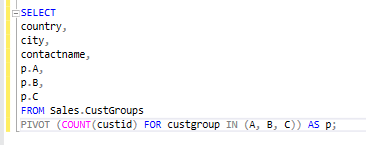
\includegraphics[width=7cm]{./Imagenes/c3}
		\end{center}
		\end{figure}
	\item Paso 3: Use una expresion de tabla común (CTE) para especificar el elemnto de agrupacion para el operador PIVOT.\\
		-  Escribir la siguiente consulta y ejecutar. 
		\begin{figure}[H]
		\begin{center}
		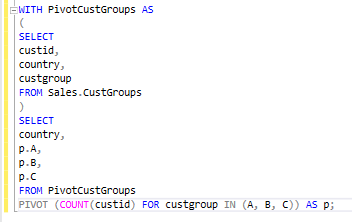
\includegraphics[width=7cm]{./Imagenes/c4}
		\end{center}
		\end{figure}
	\item Paso 4: Escribe una instruccion SELECT para recuperar el monto total de ventas para cada cliente y categoria de producto.\\
		-  Escribir la siguiente consulta. 
		\begin{figure}[H]
		\begin{center}
		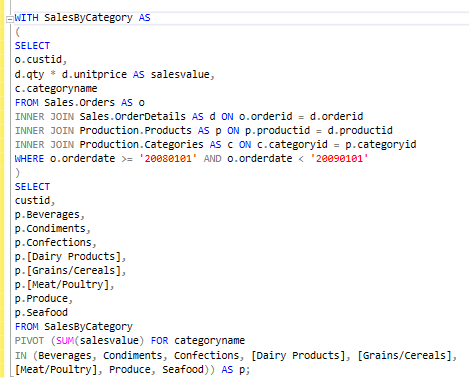
\includegraphics[width=8cm]{./Imagenes/3-2}
		\end{center}
		\end{figure}
	\end{enumerate}

	\item Escribiendo consultas con el operador UNPIVOT
	\begin{enumerate}[a)]
	\item Paso 1: Crear y consultar la vista Sale.PivotCustGroups.\\
		-  Escribir la siguiente consulta para crear una vista llamada Sales.PivotCustGroups.\\
		\begin{figure}[H]
		\begin{center}
		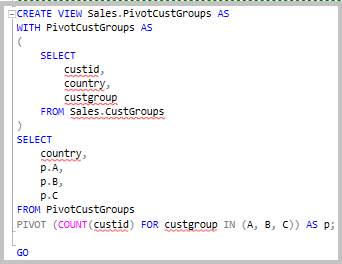
\includegraphics[width=8cm]{./Imagenes/e2-1}
		\end{center}
		\end{figure}
		-  Despues escribrir la siguiente consulta.
		\begin{figure}[H]
		\begin{center}
		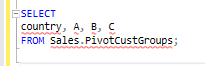
\includegraphics[width=5cm]{./Imagenes/c5}
		\end{center}
		\end{figure}
	\item Paso 2: Escriba una instruccion SELECT para recuperar una fila para cada pais y grupo de cliente.\\
		-  En el panel de consulta escribir la siguiente consulta.\\
		\begin{figure}[H]
		\begin{center}
		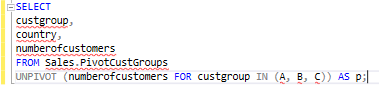
\includegraphics[width=7cm]{./Imagenes/c6}
		\end{center}
		\end{figure}
	\item Paso 3: Eliminar las vistas creadas.
		\begin{figure}[H]
		\begin{center}
		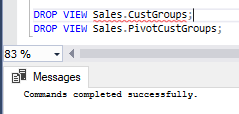
\includegraphics[width=6cm]{./Imagenes/e2-3}
		\end{center}
		\end{figure}
	\end{enumerate}



	\item Escribiendo consultas con las clausulas GROUPING SETS, CUBE, and ROLLUP.
	\begin{enumerate}[a)]
	\item Paso 1: Escriba una instruccion SELECT que use LA SUBCLAUSULA GROUPING SETS para devolver el número de
Clientes para diferentes conjuntos de agrupación.\\
		-  Escribir la siguiente consulta y ejecutar. 
		\begin{figure}[H]
		\begin{center}
		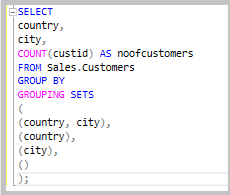
\includegraphics[width=7cm]{./Imagenes/c7}
		\end{center}
		\end{figure}
	\item Paso 2: Escriba una instruccion SELECT que use la subclausula CUBE para recuperar Grouping sets basados en valores de ventas anuales, mensuales y diarios.\\
		-  Escribir la siguiente consulta. 
		\begin{figure}[H]
		\begin{center}
		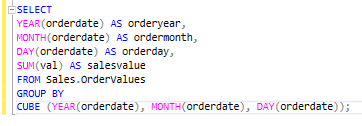
\includegraphics[width=7cm]{./Imagenes/c8}
		\end{center}
		\end{figure}
	\item Paso 3: Escriba la misma instruccion SELECT usando la subclausula ROLLUP.\\
		-  Escribir la siguiente consulta. 
		\begin{figure}[H]
		\begin{center}
		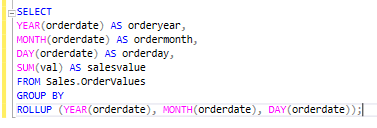
\includegraphics[width=7cm]{./Imagenes/c9}
		\end{center}
		\end{figure}
	\item Paso 4: Analizar el valor total de ventas por año y mes.\\
		-  Escribir la siguiente consulta y ejecutar. 
		\begin{figure}[H]
		\begin{center}
		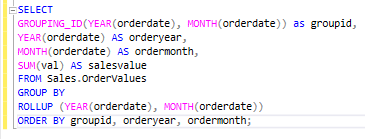
\includegraphics[width=7cm]{./Imagenes/c10}
		\end{center}
		\end{figure}
	\end{enumerate}
\end{enumerate}



